% -*- mode:LaTex; mode:visual-line; mode:flyspell; fill-column:75-*-

\chapter{Conclusions} \label{chapConclusions}

\section{Future Work}
\subsection{Design Commentary}
Much effort went into providing an important framework for the haptic to operate smoothly from a hardware standpoint but the most important progress with the final prototype was the solidification of the software framework. With the integration of delay independent state-machines performing synchronous tasks, haptic mode selection, and precise bpm control, the vibrotactile haptic could enter the next phases of development. 

The addition of BLE capability to issue commands over a paired interface such as an app on a smartphone, custom PCB to minimize form factor, and independent node abstraction of each vibrotactile could be realized. This would allow wearers capability to place a programmable array anywhere on their body enabling wide surface area dispersion and source separation. 

Lastly, experimentation with other types of vibrotactiles; either the Tactor, TacHammer, or LNA's would be more optimized for touch applications with cleaner signals, dynamic range, and optimized for skin resonance (250Hz).

\subsection{Wireless Prototype}\label{wirelessHP}
Over the course of summer of 2018, a wireless prototype was developed which eliminated the FTDI over USB interface and was completely reliant on battery power. A 9 V was connected to a voltage regulator supplying up to 5 V for the motors and 3.3V for the new MCU, sourcing up to 500 mA/hour with enough isolation to have a significantly stronger motor vibration. The MCU was based on the Particle\footnote{\url{https://www.particle.io/}} ecosystem, a cloud based IoT framework, and granted BLE and wireless capability.
\begin{figure}[H]
    \centering
    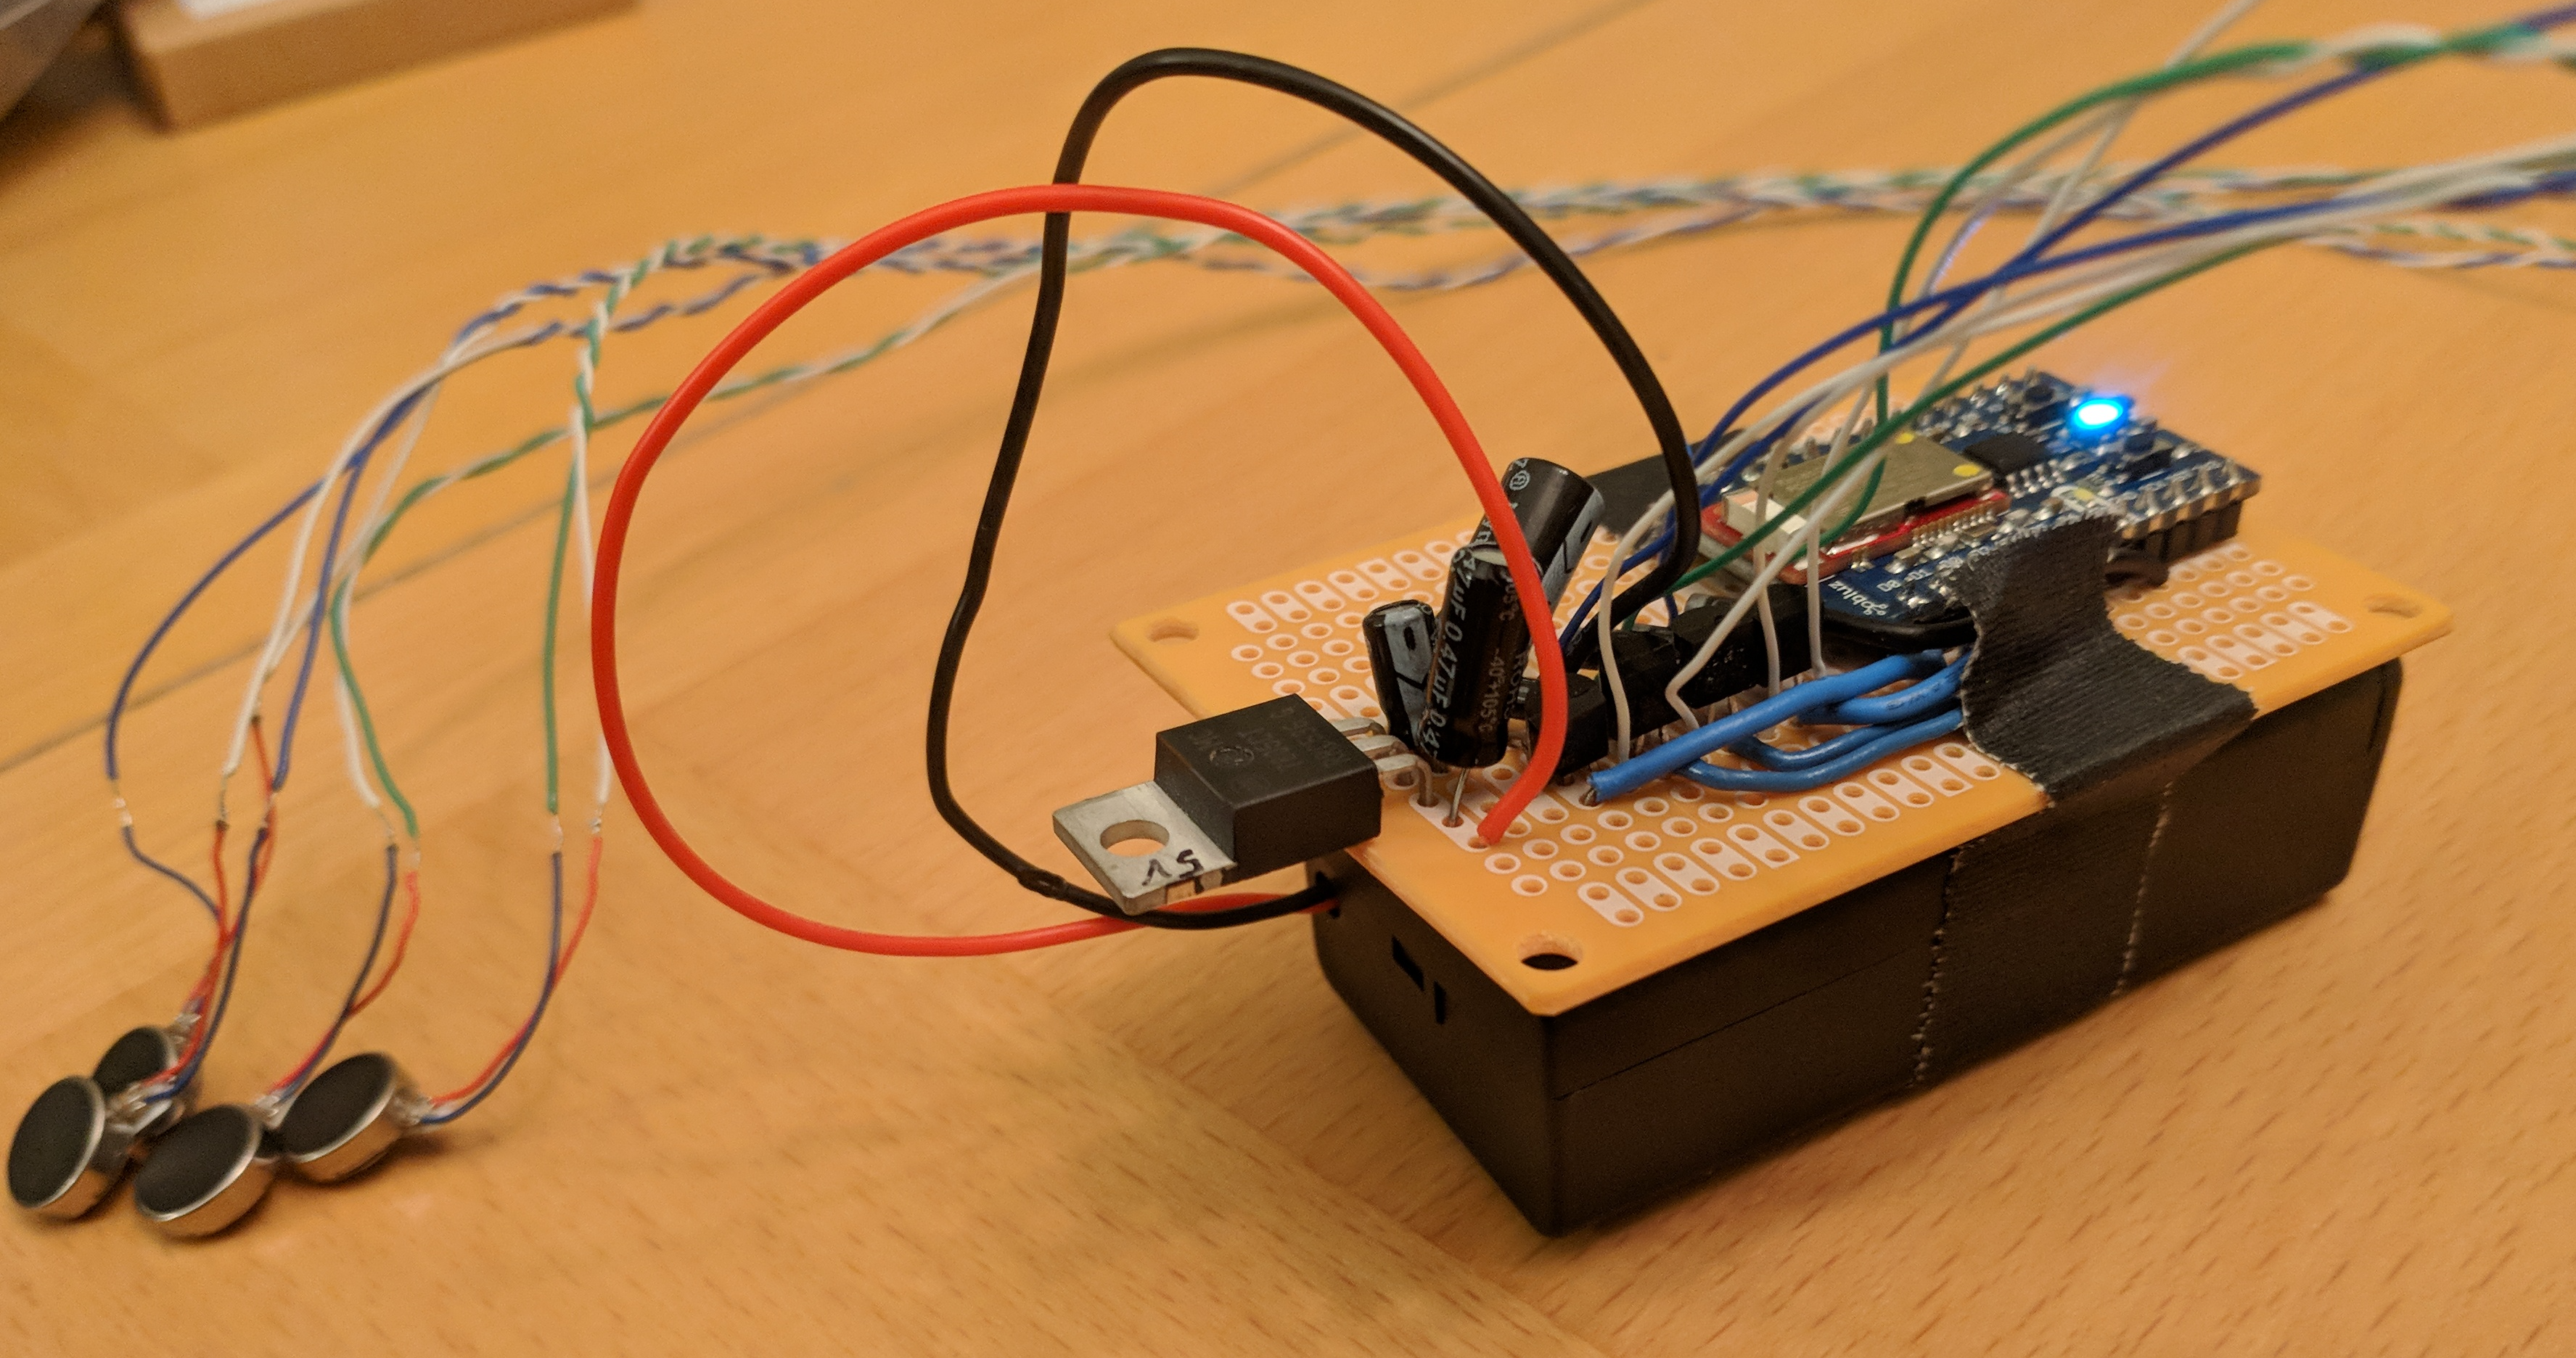
\includegraphics[width=\columnwidth]{latestProto}
    \caption{Latest wireless prototype with cloud capability}
\end{figure}
The code was altered to adapt the publish/subscribe methodology where simple numeric BPM values could be passed as API calls to the device given proper OAuth2 authentication. For example, to start the motor at 60 bpm tempo:
\begin{lstlisting}[language=html]
    curl https://api.particle.io/v1/devices/<deviceID>/motor \
       -d arg="1" \
       -d access_token=<accessToken>

    curl https://api.particle.io/v1/devices/<deviceID>/motor \
       -d arg="60" \
       -d access_token=<accessToken>
\end{lstlisting}

\subsection{Real-time Beat Tracking}
This work served as the foundational layer for the real-time beat tracking integration that is to follow. The goal is to have a haptic environmental sensing metronome, one which would intelligently adapt to the dynamics of its surroundings. Some preliminary research has been conducted to get a glimpse of the viability of such a system.

As part of the PhD work completed at the Queen Mary University of London, Adam Stark has developed a causal beat tracking algorithm intended for use in live performances\footnote{\url{http://adamstark.co.uk/project/btrack-a-real-time-beat-tracker/}}\cite{stark2009real}. The real-time beat tracking results were comparable to top of the line non-causal systems. The algorithm was initially implemented in C++ with wrappers for Python but externals were later made available for Max/MSP.
The Max patch was expanded to fit the context of this work. In doing so the patch was retrofitted to send instantaneous BPM signals over serial thus communicating with the haptic device shown in Figure \ref{fig:BTMaxPatch}.

\begin{figure}[H]
    \centering
    \includegraphics[width=\columnwidth]{BTMaxPatch}
    \caption{Beat tracking max patch with additions for sending bpm over serial}
    \label{fig:BTMaxPatch}
\end{figure}

This was an important step to determine feasibility. Though some phasing occurs do to the jittery nature of the \textit{btrack} patch, some intelligent averaging is necessary to lock to a bpm. Work in the future can expand on this conceptually and also provide some windowing or system wide delay to provide further synchronization.

\subsection{Extra-musical Applications}
The same researchers who developed the haptic drumkit discovered the extension of the application towards those with restricted mobility such as stroke patients and those suffering from Parkinson's disease. The results were promising, one patient who was a veteran mentioned that it put a marching sense back into his mind and helped remind him of the sensation of even walking. They morphed the project into what is known now as the haptic bracelet 4 years later \cite{holland2014gait}.

This work has hope to move in the same direction with a system giving constant feedback to inform the wearer of upcoming obstacles and help usher through dynamically changing thresholds.